\documentclass{ijuc}
\usepackage[pdftex]{graphics}
\usepackage{graphicx}
\usepackage{amssymb}

\begin{document}

\title{Combinatorial approach to counting equivalence classes in 1D and 2D cellular automata}
\author{Iztok Jeras\inst{1}\email{iztok.jeras@rattus.info}}
\institute{Faculty of Computer and Information Science, University of Ljubljana, Slovenia}
\def\received{Received 17 December 2004; In final form 1 April 2005}

\maketitle

\begin{abstract}
There is much more theoretical research on 1D cellular automata compared to 2D.
While not the main reason one of the arguments given is that the number of
available rules for a common 2D neighborhood is too large for a comprehensive
analysis. This issue can be mitigated by focusing on the smallest 2D neighborhoods
(trid and quad) and by grouping rules into equivalence classes. This article
gives an algebraic combinatorial solution to counting equivalence classes.
\end{abstract}

\keywords{cellular automata, combinatorics, equivalence classes, congruence operations}

\section{Introduction}

This describes the IJUC \LaTeX\ style
class file {\tt ijuc.cls} and the Bib\TeX\ file {\tt ijuc.bst},
suitable for processing with {\tt latex} or {\tt pdflatex}.
(This example file has a pdf figure example,
so should be processed with {\tt pdflatex}.)

\section{Formalization}

\section{Definition of Equivalence}

\subsection{1D problem}

Mention of figures and tables within text: When referring to figures, tables
and other elements within the text, always call the element by its full name (for
example: ``See Table 1,'' ``Figure 1 illustrates\ldots,'' ``Refer to Scheme 1.'' Do not
use ambiguous phraseologies (for example: ``1 illustrates\ldots'') that do not clearly
denote the element being referred to.


\subsubsection{Counting neighborhoods}

The set of all distinct neighborhood values for a given neighborhood size and number of cell states is:

\[ \mathbb{M} = \left\{ n : \right\} \]
\[ \vert \mathbb{M} \vert = k^m \]

Neighborhoods can be organized into subsets depending on their invariance to congruence operations.

There are neighborhoods which are invariant to reflection:

\[ \mathbb{M}_\mathrm{ref} = \left\{ \forall n \in \mathbb{M} : \phi_\mathrm{ref}(n) = n \right\} \]
\[ \vert \mathbb{M}_\mathrm{ref} \vert = \left\{ 
  \begin{array}{ll}
    {k^{m/2+1}} & \quad \textrm{if $m$ is odd }\\
    {k^{m/2  }} & \quad \textrm{if $m$ is even}
  \end{array} \right.
\]

There are no neighborhoods which are invariant to permutation:

\[ \mathbb{M}_\mathrm{per} = \left\{ \forall n \in \mathbb{M} : \phi_\mathrm{per}(n) = n \right\} = \varnothing \]
\[ \vert \mathbb{M}_\mathrm{per} \vert = 0 \]

There are neighborhoods which are invariant after both reflection and permutation have been applied:

\[ \mathbb{M}_\mathrm{ref,per} = \left\{ \forall n \in \mathbb{M} : \phi_\mathrm{per}(\phi_\mathrm{ref}(n)) = n \right\} \]
\[ \vert \mathbb{M}_\mathrm{ref,per} \vert = \left\{ 
  \begin{array}{ll}
    {0        } & \quad \textrm{if $m$ is odd }\\
    {k^{m/2  }} & \quad \textrm{if $m$ is even}
  \end{array} \right.
\]

\subsubsection{Counting rules}

Tables are numbered consecutively and should include a clear
descriptive caption (see Figure \ref{fig-eg}).

\begin{figure}
\begin{center}
\scalebox{0.5}{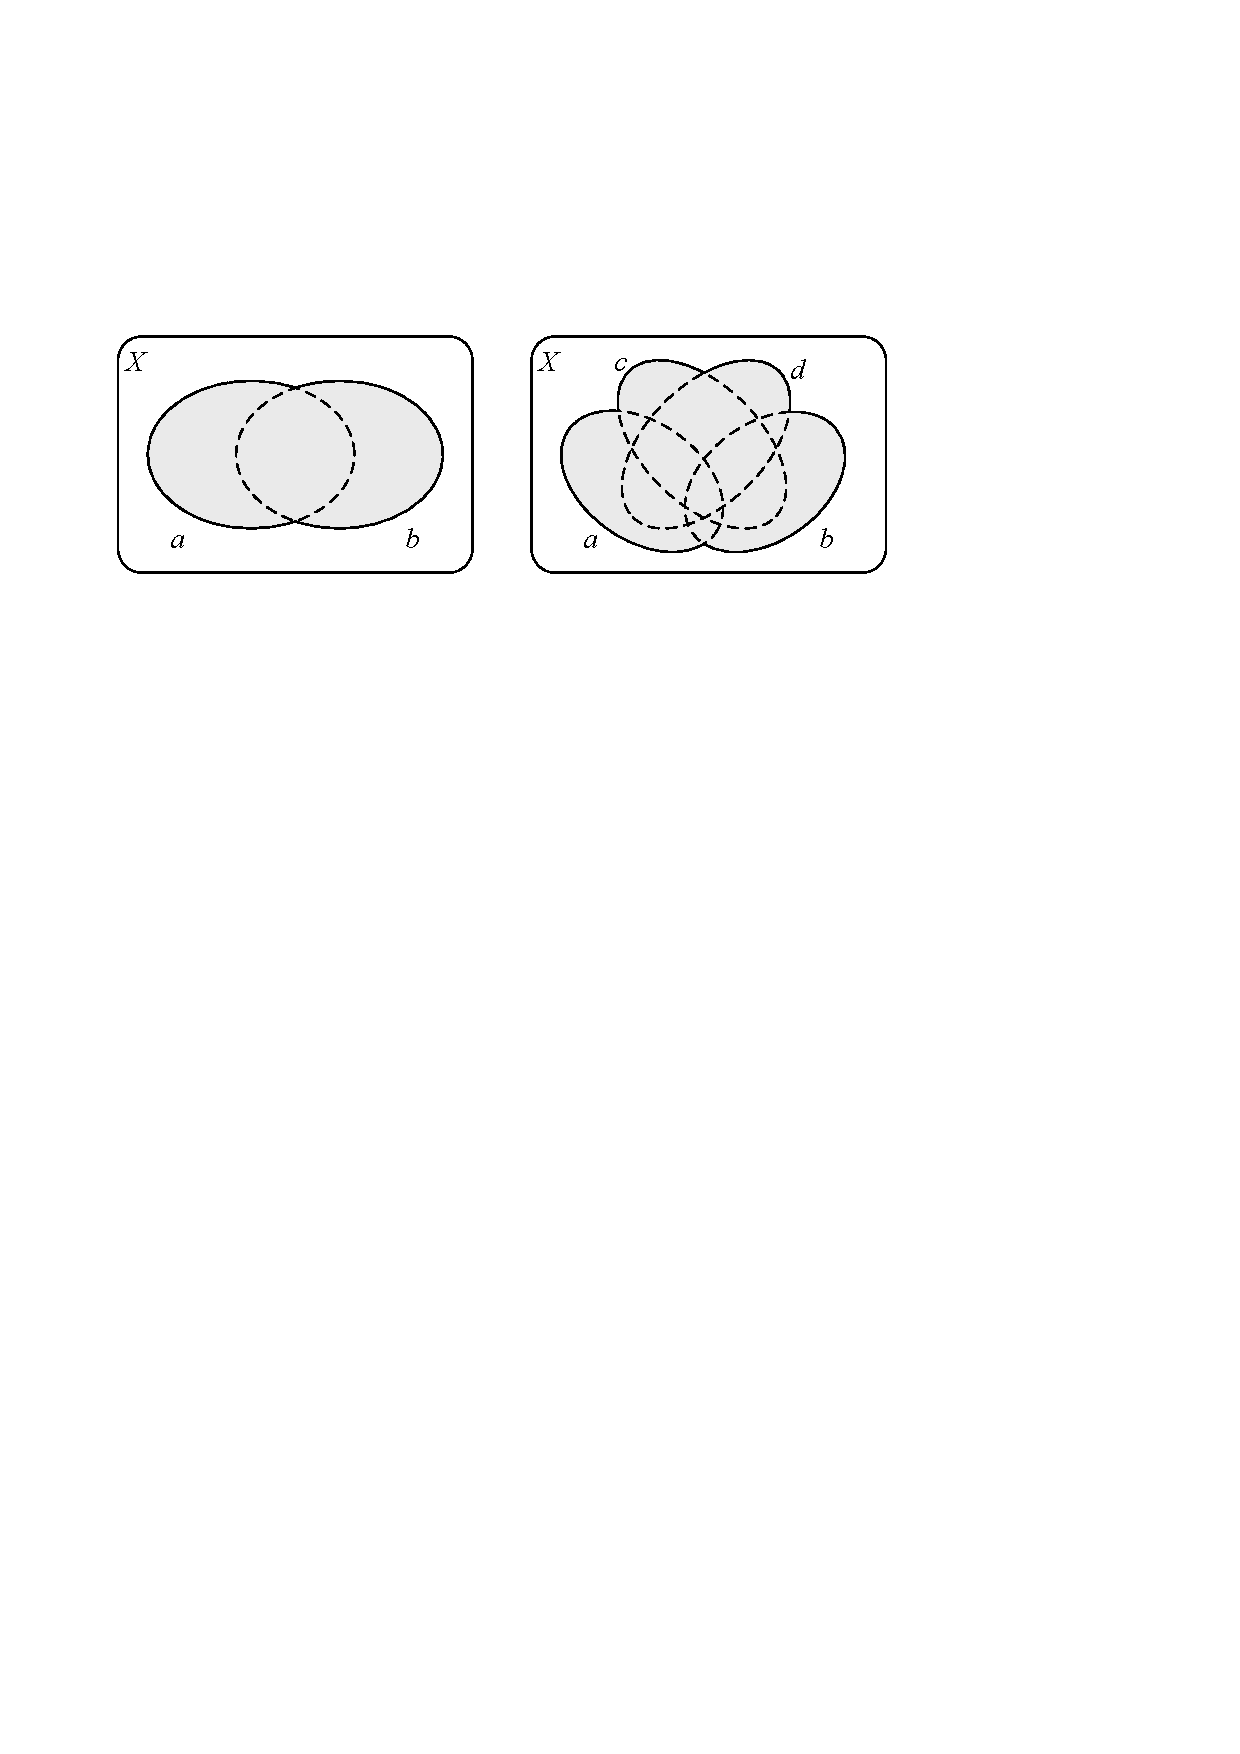
\includegraphics{union.pdf}}
\end{center}
\caption{Example figure, taken from reference \cite{St1}.}
\label{fig-eg}
\end{figure}




\subsubsection{Tables}

Tables are numbered consecutively and should include a clear
descriptive caption. Avoid the use of structural formulas in the body
of tables. Table footnotes should be given a footnote symbol as explained in
the Footnotes section, proceeding by row rather than by column order.
Footnotes within a table should be indicated by the same
symbols listed above. Reinitialize symbol sequence within tables. Place footnotes
to a table directly beneath the table. (See Table \ref{tbl-eg}).


\begin{table}
\begin{center}
\begin{tabular}{|@{\hspace{1mm}}c@{\hspace{1mm}}|c||c|c|@{\hspace{1mm}}c@{\hspace{1mm}}|}\hline
$X$ range&$R$ values&$\alpha$ \footnotemark[1] & $\mathit{MIL}$ \footnotemark[2]& $\mathit{MaxIL}$\\\hline
$-8$:20:2& 2.5, 3.0&0.97\footnotemark[3]&500&500\\\hline
$-8$:30:2&2.5&0.98&1000&1000\\\hline
\end{tabular}
\end{center}
\caption{Example table, excerpted from reference \cite{St2}.\\
{\footnotesize
\footnotemark[1]a footnote about $\alpha$;
\footnotemark[2]in row not column order;
\footnotemark[3]the last footnote
}
} 
\label{tbl-eg}
\end{table}



\subsection{Footnotes}

Authors are encouraged to minimize the use of footnotes. A
footnote may include the designation of a corresponding author of the paper,
current address information for an author (if different from that shown in the
affiliation), and traditional footnote content. 


Footnotes are indicated in the text by the following symbols:
asterisk\footnote{asterisk or star},
dagger\footnote{dagger}, 
double dagger\footnote{double dagger}, 
paragraph mark\footnote{paragraph mark}, 
section mark\footnote{section mark}, 
parallels\footnote{parallels}, 
number sign\footnote{number sign},
and then their doubled counterparts. 

Numerals are not used for footnote callouts,
as they may be mistaken for bibliographical reference call-outs or exponents.


\section{Acknowledgments}

Information concerning grant
support of research should appear in a separate Acknowledgments section at
the end of the paper, not in a footnote. Acknowledgments of the assistance of
colleagues or similar notes of appreciation also properly belong in an
Acknowledgments section, not in footnotes.


\section{Citing References}

References are indicated in the text by consecutive Arabic numbers
in brackets. The full list is collected at the end of the paper in numerical
order. All references in the list should be cited within the text, and vice
versa. Listed references should be complete in all details, including article
titles in journals. All authors on each paper should be cited; ``et al.'' is not sufficient.
Journal title abbreviations should conform to Mathematical Reviews
Index style.


\bibliography{equivalence}

\appendix 

\end{document}
